% Selected DSN2027 manuscript; evidence and release provenance are archived separately.
\documentclass[conference,10pt]{IEEEtran}
\usepackage[T1]{fontenc}
\usepackage{cite,amsmath,amssymb,amsthm}
\usepackage{booktabs,array,multirow,graphicx}
\usepackage{url,microtype}
\usepackage[hidelinks]{hyperref}
\newtheorem{definition}{Definition}
\newtheorem{proposition}{Proposition}
\begin{document}
\title{RevTrace: Preserving Valid Progress across Trusted Feedback Revisions}
\author{\IEEEauthorblockN{Anonymous submission}\IEEEauthorblockA{Regular paper}}
\maketitle
\begin{abstract}
Trusted feedback can invalidate speculation without invalidating all of its
computation or delivered progress. RevTrace composes dependency reuse and
whole-hypothesis consumption around a protected feedback-state contract.
Complete frozen inputs provide executable eligibility witnesses; compatible
certified updates preserve supported ahead views while original selection
retains write authority. A native implementation confirms inputs of already
executing full recognizer--corrector calls without requiring their own next
predictions to be correct. In a predeclared 24-speaker ASR stratum,
computation-only retention increases frontier withdrawals from 12 to 17;
joint coordination produces zero and adds 26.645 seconds of deadline credit
over 714.110 seconds offered. On four previously unused native speakers,
full-call retention meets both whole-run deadlines in eight of eight runs
versus zero for conservative execution, preserving complete original
correction histories. A 48-run workload study separates
timely first delivery from subsequent availability and identifies measured
service boundaries.
\end{abstract}
\begin{IEEEkeywords}
dependable inference, feedback state, incremental computation, speculative execution, streaming ASR
\end{IEEEkeywords}
\section{Introduction}\label{sec:intro}
Feedback-driven speech recognition repeatedly turns generated text into
input for later inference. A trusted correction can improve the current
transcript and change the state from which the next recognition starts.
This makes each correction an execution boundary: some ongoing speculative
work has become invalid, while other work may still be a valid continuation.
A dependable service must distinguish these cases while delivering useful
progress before its trusted path catches up.

An execution from our prototype exposes the problem. A complete hypothesis
covering a two-second audio interval reached the actual Consumer 1.444~s
after that interval became available, meeting its two-second display
deadline. At 1.544~s, a new certified result replaced the visible view with
a shorter snapshot. The discarded hypothesis still had a valid dependency
path from the new feedback state. It remained absent at the original
two-second deadline and returned at 3.720~s through certified delivery,
within its eight-second deadline and with exactly the same text. The
temporary loss removed 37 newly displayed characters, including spaces.
Both first-delivery deadlines were met, yet already delivered valid progress disappeared for
2.176~s. This is a loss of interval coverage under a compatible update,
independent of whether the provisional transcription is semantically correct.

\begin{figure*}[t]
\centering
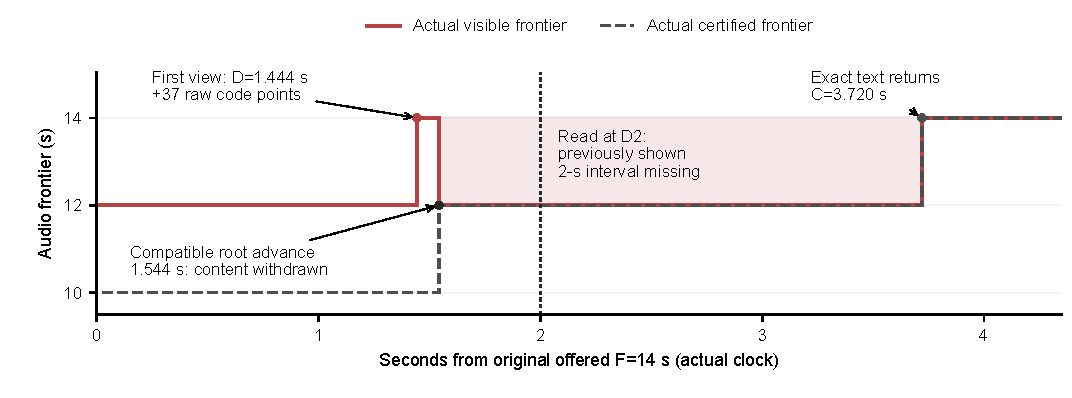
\includegraphics[width=\textwidth]{figures/timely_full_interval_case.pdf}
\caption{An actual interval in the computation-only arm. First display meets
D2 and certified delivery meets C8, yet a compatible root update withdraws
the newly displayed phrase for 2.176~s. The dotted line samples the actual
view at the original D2 deadline. This explanatory case comes from the
c16 workload, whose whole-run D2 P99 fails; it is not a paired
counterfactual or an estimate of natural prevalence.}
\label{fig:continuity_case}
\end{figure*}

Computation retention alone can exacerbate this mismatch. In our
predeclared Qwen evaluation on three new eight-speaker cohorts, retaining
valid computation improved timely delivery but increased observed
audio-frontier withdrawals from 12 to 17 when the Consumer still installed
snapshots. Retaining the computation and its compatible whole view together
produced zero frontier withdrawals in that stratum. The issue is therefore
how valid work becomes sustained service across a trusted update, as well
as how quickly the work finishes.

There are strong foundations for this design. Incremental dialogue models
already distinguish active and committed information and propagate
revocation~\cite{schlangen2011incremental}; incremental computation reuses
work through dependencies and stable identities
\cite{hammer2014adapton,hammer2015names,mcsherry2013differential}.
SSBD coordinates old draft reuse with display-only masking in
re-translation~\cite{zeng2026ssbd}, and PredGen speculates on downstream
responses while speech input evolves~\cite{li2025predgen}. We apply these
ideas to a protected feedback contract in which the original trusted
selection recursively supplies later ASR inputs. The contract governs two
decisions: whether executed work remains eligible under the new root, and
whether installing that root preserves the Consumer's current whole
hypothesis. Separate sufficient guards enforce the feedback dependencies
at these boundaries. Together they provide conditional continuity of
already delivered progress while retaining selection authority and
necessary revisions.

RevTrace reconciles executed calls and delivered whole hypotheses with each
new trusted feedback state. A call remains eligible when its complete frozen
input has a valid dependency witness from that state; the Consumer separately
checks whether its current whole hypothesis remains supported. These
decisions retain work and service while original protected selection
determines the next feedback state. We instantiate the same eligibility
principle with recorded continuation paths in the core runtime and with
input-confirmed full calls in a native correction pipeline. Work with no
remaining use follows a separate coverage rule, and its physical lease ends
only after actual drain.

This paper makes three contributions:
\begin{itemize}
\item A feedback-state contract and executable sufficient witnesses for
  retaining owned computation across trusted updates, including recorded
  continuations and input-confirmed full calls. These witnesses bind
  complete state, actual audio frontiers, frozen inputs, and execution
  identity.
\item Joint coordination of computation and whole Consumer views, with a
  conditional guarantee that applying a compatible certified root does not
  itself withdraw an ahead view. Necessary revisions remain permitted.
\item An implementation and service evaluation that hold the selected
  feedback task fixed. Factorial controls isolate computation and whole-view
  retention; a published native correction pipeline tests whether
  input-confirmed full execution improves timely service while preserving
  original correction and complete state transitions.
\end{itemize}

In the independent headline stratum, the joint design adds 26.645~s of
original dual-deadline credit over 714.110~s offered audio while preserving
the complete certified histories. A separate 48-run workload study shows
where the arms converge and where deadline pressure remains, including a
negative intermediate-load confirmation. Subsequent-availability analysis
keeps its own definition and leaves the original first-delivery metrics
unchanged. A separately frozen native confirmation on four previously
unused speakers raises credit from 37.0 to all 66.340~s offered per arm
and whole-run D2/C8 passes from zero to eight of eight runs.
The core study isolates whole-view continuity; the native study tests
timely execution of the unchanged original feedback task.

\section{Feedback Contract}\label{sec:contract}
\subsection{Feedback creates an execution dependency}
Consider a service that receives an immutable audio stream and repeatedly
uses generated output as input to later recognition. A protected selection
path produces \emph{Canonical} facts. A faster \emph{Private} path may
compute and display provisional hypotheses while selection is pending.
The selected correction can change the state consumed by the next call:
StreamCorrect, for example, feeds its chosen correction back into subsequent
ASR~\cite{vu2026streamcorrect}. The problem is to coordinate this dependency
while the two paths advance asynchronously.

For a fixed session and execution contract, write an installed fact as
\begin{equation}
 C=(v,F,Z_C,P_C,T_C).
 \label{eq:canonical}
\end{equation}
Here $v$ is its version, $F$ its certified audio frontier, $Z_C$ the complete
selected output, $P_C$ the feedback state for later calls, and $T_C$ its bound
display text. A contract specifies the model, adapter, decoding configuration,
audio identity, and transformations from a complete output to $P$ and $T$.
Here $F$ is a state-processing boundary. Consumer coverage follows the
adapter's publication policy; advancing $F$ need not add visible characters.
Certification means that the protected selection and installation protocol
accepted this fact. Recognition accuracy against human transcription is a
separate property.

The adapter declares a conservative representation of \emph{all mutable
cross-call state that can affect later model inputs, selection, or feedback}.
Telemetry and device resources are recorded separately. The Qwen adapter passes prompt
tokens between calls and carries no numerical KV cache across them. The
native correction adapter additionally carries audio buffers, token groups,
context, alignment position, and decoder configuration. A state comparison
is meaningful only within its declared contract: text equality cannot stand
in for an unrecorded alignment cursor or numerical cache. The representation
may include more fields than a particular next call needs; we do not require
it to be minimal.

\subsection{Three lifetimes of provisional work}
A complete provisional node $n$ records a frozen call
\begin{equation}
 q_n=(a_n,P_n^-,b_n,\chi_n),\quad
 n=(q_n,Z_n,P_n^+,T_n),
 \label{eq:node}
\end{equation}
where $a_n$ is the input-state frontier, $b_n>a_n$ the target audio frontier,
and $\chi_n$ binds the remaining inputs and execution identity. The model
may read the complete audio prefix through $b_n$; $a_n$ does not claim a
token-to-audio alignment. $P_n^+$ and $T_n$ are derived from the complete
result through the contract's adapter. An in-flight call has a frozen input
and no complete output yet. Partially generated or cancelled tokens cannot
become a complete node.

Such work has three distinct lifetimes. Its \emph{dependency lifetime}
determines whether it can still be used under the current Canonical root.
Its \emph{visible lifetime} determines whether the Consumer keeps its whole
published hypothesis. Its \emph{physical lifetime} ends when the executor
has actually finished or drained the work. A new root can change the first
two without immediately ending the third. RevTrace connects their decisions
while keeping the evidence for each decision explicit.

The service retains every accepted input obligation until certified
processing covers it. Discarding a branch, requesting cancellation, or
recovering an old view does not remove that obligation or reset its arrival
clock. In exact mode, a missed deadline never authorizes an uncertified
Canonical transition.

\subsection{Trust and failure boundary}
We assume one trusted Owner per session, a protected selection path,
immutable accepted audio and model configuration, unambiguous encoding,
collision-resistant digests, and storage that honors successful
synchronization. Calls used in the dependency argument must actually consume
their frozen inputs and return the corresponding complete results. This
execution-integrity premise is explicit: host receipts and text hashes bind
API objects; they are not GPU arithmetic attestation. Private and Authority
need not return identical results from independent floating-point executions.

At its declared interface, the runtime checks result identity, completeness,
derived-state consistency, and ancestry, including late or repeated messages.
Provisional content can still be inaccurate. The separately frozen recovery configuration
handles whole-process termination on the same intact filesystem.
A compromised coordinator or Authority,
Byzantine host code, arbitrary persistent corruption, and lost storage are
outside this boundary. The controlled wrong-input injections in
Section~\ref{sec:eval} intentionally violate normal Private input fidelity;
we use them to study containment and executor release, not as examples
covered by the lawful-continuation proposition.

\section{Valid Continuations and Whole Views}\label{sec:continuation}
\subsection{A continuation under a new root}
The central question is whether an old call still belongs to a valid
provisional continuation after trusted feedback advances. Its birth version
records dispatch history. The dependency witness establishes whether it
remains usable now.

Let $x=(F,P_C)$. A complete recorded node provides an edge
\begin{equation}
 (F,P_C)\xrightarrow{n}(b_n,P_n^+)
 \quad\text{if}\quad a_n=F\ \land\ P_n^-=P_C,
 \label{eq:edge}
\end{equation}
under the input, identity, and execution contract of
Section~\ref{sec:contract}. A finite sequence of such edges is a
\emph{valid provisional continuation} of $C$ when each successor consumes
the preceding complete output state at its actual frontier. Write
$C\leadsto n$ for a complete path to $n$. A frozen in-flight successor can
belong to the same continuation, but contributes no usable result until
completion.

\begin{proposition}[Sufficient re-rooting witness]
\label{prop:rebase}
Suppose an old branch contains a complete boundary node at the new certified
frontier $F$, with output state $P_C$. If its subsequent recorded calls form
an unbroken input--output path to the actual branch tip, those nodes are a
valid provisional continuation of $C$. An in-flight successor may continue
when its unchanged frozen input is that tip and its target exceeds $F$.
\end{proposition}
\begin{proof}
The boundary node provides $(F,P_C)$, equal to the new root's declared
cross-call state. The first successor therefore satisfies
Eq.~\eqref{eq:edge}. Inductively, each next call consumes the preceding
complete output at its recorded frontier, with the remaining inputs bound
by the same contract. The path reaches the actual tip. The in-flight
successor satisfies the next input edge, without yet supplying an output.
Re-rooting changes none of these calls or their frozen inputs.
\end{proof}

This establishes dependency validity. The provisional result remains subject
to later selection and revision; re-rooting grants no Canonical write
authority. The argument also makes no bitwise-replay assumption for a
different floating-point execution. Its witness follows calls that actually
occurred.

Two short counterexamples explain the required observations. A branch born
under $v$ may reach exactly $(F,P_C)$ when $v+1$ is installed; discarding it
solely because its version is older loses a valid continuation. Conversely,
equal displayed text can hide different feedback tokens or alignment state.
A call consuming one state has no valid path from the other merely because
their text agrees. Equal state at a different audio frontier likewise does
not provide Eq.~\eqref{eq:edge}.

\subsection{Retaining computation: \texorpdfstring{$R$}{R}}
In the core Qwen implementation, the computation guard implements a conservative witness for
Proposition~\ref{prop:rebase}. On a Canonical installation, it first finds a
complete Private node at exactly $F$ whose full feedback tokens equal
$P_C$. It follows complete successors, checking each frozen input and
frontier, until it reaches the recorded branch tip. An intermediate match
cannot stand in for a path to that tip. If a successor is in flight, the
guard requires the unique tracked task to consume this tip and target
audio beyond $F$.

When the witness succeeds, the Owner retains the branch and updates its
eligibility relative to the new root. The original job identifiers, birth
versions, input tokens, and results remain unchanged. Otherwise it fences
the continuation lacking this witness and rebuilds from an allowed state. This
guard's boundary-node and unique-slot requirements restrict what this
implementation can retain; they are not universal necessities for every
valid reuse scheme.

\subsection{Retaining an actual view: \texorpdfstring{$S$}{S}}
Computation retention alone does not preserve service that has already
reached the Consumer. A snapshot Consumer can replace an ahead view with
the newly certified, shorter view even when the ahead computation is still
valid. RevTrace instead maintains a certified lane and a provisional lane.
Both hold whole hypotheses; there is no uncertified suffix splice. The
Consumer records the certified text and provisional visible text separately,
so a retained provisional view acquires no certified-prefix status.

On applying a new Canonical publication, $S$ checks the complete currently
visible provisional node. It can prove a path directly when that node's
frozen input is $(F,P_C)$, or follow its complete published ancestors to
that boundary. Missing, cyclic, or ambiguous ancestry is rejected. This
check uses the same feedback-state contract as $R$, while accepting a
different sufficient witness: a directly rooted published call does not
need an extra Private boundary node.

The Consumer first previews the whole next view. The protocol kernel then
checks the installed durable root, actual registered results, dependency
path, and bound text/frontier before authorizing the actual application.
Only that application yields the recorded view receipt. A caller-supplied
compatibility flag cannot replace the underlying nodes.

\begin{proposition}[Continuity at a compatible application]
\label{prop:continuity}
Immediately before an authorized Canonical application, let the visible
whole provisional view $h$ be ahead of its new frontier $F$. If $S$ proves
$C\leadsto h$ and no independent withdrawal mode is invoked, that
application advances the certified lane and preserves $h$ unchanged.
\end{proposition}
\begin{proof}
The compatible-and-ahead branch installs $C$ into the certified lane and
retains the existing provisional node, text, and frontier. The kernel
authorizes this preview against the actual root and complete dependency
records before the Consumer applies it. Thus this application does not
itself withdraw any part of $h$.
\end{proof}

An incompatible update must still withdraw the view. Later valid results
can also revise text or replace a hypothesis. Consequently the property
concerns one compatible root application, rather than global monotonic
display. Snapshot-only service and conservative recomputation can be safe;
the four-arm experiment asks what additional progress $R$ and $S$ preserve
together, and where that benefit is worth its cost.

% Integrated core working draft; final independent-source research and release QA pending.
% Evidence scope: original packet controls and actual full-call service; no encoder-cache result.
\subsection{Native feedback and conditional full calls}
\label{subsec:native_full_calls}
StreamCorrect's original recognizer, learned correction, and feedback update
provide a concrete instance of the contract in Section~\ref{sec:contract}
\cite{vu2026streamcorrect}. Let $P$ be a complete closed native state and
$X$ the next accepted audio input. We expose the recognition boundary as
\begin{equation}
  A(P,X)=(B,M),
\end{equation}
where $B$ contains the ordered beam candidates and $M$ contains the live
engine state and inputs required by the remaining correction and update.
The protected original $C/U$ selects a correction and produces the next
closed state. Its selection, candidate order, prompts, returned token IDs,
and update rules remain intact.

Before that selection finishes, the original update tail supplied with a
typed first-beam identity prediction produces a provisional closed state
$\widehat P^+$. This projection has explicit provenance: recognition has
executed, but learned correction has not completed for this projected node.
It supplies a conditional input for the next complete call. Both GPUs host
the original full recognizer--corrector pipeline, so a call dispatched on
this input executes the protected original $C/U$ as well. Completed
conditional full results and typed identity projections remain distinct
objects. Neither is installed merely because its predicted text looks
plausible.

When the selected parent arrives, the Owner compares the call's entire
frozen start state, actual frontier, execution contract, and session epoch
with the installed parent. An exact match confirms the already owned call:
an in-flight call continues, or an already completed result becomes eligible
for ordered installation. The job's birth root, identifier, epoch, inputs,
and execution history are unchanged. The call's own identity prediction need
not equal its eventual corrected output; confirming its input establishes
eligibility, while original correction determines its result.

An earlier ancestor mismatch removes support for the tracked provisional
chain, but does not prove that a later complete input cannot converge.
Cancellation before correction therefore requires an actual selected state
at the call's same start frontier that disagrees with its complete input,
coverage of its target without remaining use, or a changed epoch. A still
unresolved future parent supplies none of these proofs.

This direct native witness instantiates the continuation relation of
Section~\ref{sec:continuation}. It differs from the core Qwen computation
guard, which conservatively requires an explicit matching boundary node and
a uniquely tracked successor. These are different sufficient implementations
of eligibility. The whole-view Consumer likewise keeps certified and
provisional provenance separate and applies complete supported hypotheses.
We compare conditional full-call retention with an already-ready ASR packet
alternative. Both are author-built implementations of the same feedback
principles; the measured native benefit concerns confirmed complete calls.

\section{Execution Protocol}\label{sec:protocol}
\begin{figure*}[t]
\centering
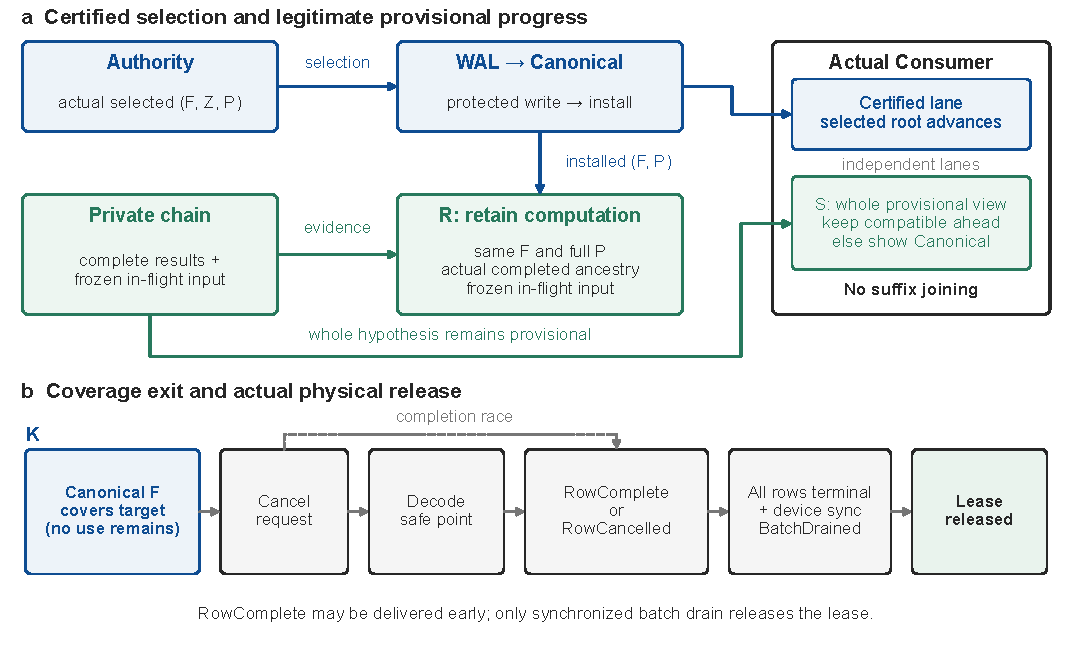
\includegraphics[width=\textwidth]{figures/coordination_protocol.pdf}
\caption{RevTrace coordinates complete provisional computation and whole
Consumer views with certified state. $R$ and $S$ use the same declared
feedback dependencies, with separate sufficient guards. Coverage retirement
uses a different predicate. A complete result may be consumed before its
batch drains; only terminal rows plus device synchronization release the
physical lease.}
\label{fig:protocol}
\end{figure*}

\subsection{Complete results and physical ownership}
This section describes the core ASR runtime. The native correction adapter
uses its separately declared full-state interface; its validation does not
inherit the core kernel's recovery or physical-lease evidence automatically.
Figure~\ref{fig:protocol} separates publication from physical completion.
Each dispatch binds a session, worker incarnation, job, frozen input, target
frontier, and execution contract. The wrapper accepts only an exclusive
complete-row or cancelled-row outcome. It re-derives feedback state and
text from the bound complete result. A cancelled row reports accounting
information and supplies no partial feedback state.

The Owner can validate, durably install, and publish a complete row while
other rows of its physical batch are still running. This prevents a
completed session from inheriting another row's entire completion delay.
Physical ownership has a separate condition: every row must have a terminal
outcome and the device must synchronize before \texttt{BatchDrained}
releases the batch lease. A complete publication alone cannot authorize
reusing the executor.

\subsection{Covered work and safe-point exit: \texorpdfstring{$K$}{K}}
An old birth version does not determine either usability or uselessness.
For the tested use model, $K$ requests exit when the actually installed
Canonical frontier covers a proposal's target and that work has no
remaining declared use. This coverage predicate answers a different question
from $R$: a valid continuation beyond the new root may still be useful.

\texttt{CancelRequest} is a request, not a completion event. The worker
observes it at supported decode boundaries. Completion can win the race;
the runtime records either a complete result or cancellation, never both.
It waits for all row terminals and actual drain before releasing the lease.
The static batch is not compacted or refilled, and residual cost for masked
rows remains in the measurements. The protocol supplies no arbitrary-GPU
millisecond cancellation guarantee. Its service value is the measured
execution window available to subsequent lawful work.

\subsection{Durable facts and outstanding input}
Canonical state and transition identity are synchronized before a successful
acknowledgment. Each journal frame binds the parent and next state, request
identity, selected complete result, and receipt. The runtime verifies that
the recorded delta reconstructs the proposed state. Group-ready commit
shares a synchronization barrier among already validated transitions of
different sessions; it introduces no collection timeout and no cross-session
all-or-nothing transaction. An uncertain append or state-application outcome
blocks further writes until recovery.

Recovery validates framing, checksums, state chaining, and contracts, then
reconstructs certified state and admitted identities. An identical retry
retrieves its recorded outcome; a changed request with the same identity
conflicts. These are conventional write-ahead recovery principles
\cite{mohan1992aries} instantiated at the feedback boundary.

In the recovery configuration, the recovered view can be applied before cold neural workers finish
loading. This restores existing service facts, not progress on new audio.
The input journal separately preserves accepted but uncertified audio and
its original clocks, so replaying old text cannot discharge new work.
Process epochs fence old workers and publications. These checks rely on
exclusive ownership and intact synchronized storage, as declared in
Section~\ref{sec:contract}.

\subsection{Validation boundaries}
The re-rooting argument and conditional view property are supported by
targeted source-level witnesses and actual service interleavings.
Separately, bounded exploration of an earlier recovery prototype covers
durable-root, view-application, and physical-lease interleavings. Its
1,154-state single-session product does not represent the full multi-node
re-rooting guard or an arbitrary neural execution. We therefore use it as
component-level protocol evidence, with its own frozen source, rather than
a complete machine proof of Propositions~\ref{prop:rebase}
and~\ref{prop:continuity}.

A separately frozen recovery prototype completed 84 GPU service runs:
24 normal, 36 process-group SIGKILL, 16 controlled-boundary, and eight
post-sync crashes. The 44 crash audits recorded no acknowledged-input loss.
All 32 early-recovery crash runs reapplied old facts before workers were
ready. In one Qwen configuration, median old-view recovery changed from
31.013 to 14.736~s; first new certified output still took 33.829~s.
The complete-composition control shared the benefit. All 44 crash runs
missed whole-run D2/C8. These are earlier-prototype measurements, not fault
validation of the current core or native adapter.

\section{Evaluation}\label{sec:eval}
\subsection{Experimental design and service endpoints}
We evaluate two service obligations under unchanged selected feedback
histories: retaining dependency-valid progress already at the Consumer,
and completing selected transitions before their original deadlines.
The core factorial study isolates computation and whole-view retention;
the native study tests input-confirmed full execution of the original
correction pipeline. Timing, content support, and energy remain separate.
The core experiments use actual neural
calls, durable input and Canonical journals, and an instrumented FIFO
Consumer. Measurements use Consumer applications rather than publication
or display replay. Accepted input obligations retain
their original arrival clocks.

\paragraph{Implementation and workloads}
The service uses two 24-GB RTX~3090s: an FP16 Private worker and an FP32
Authority worker. Qwen3-ASR~1.7B~\cite{shi2026qwen3asr} is the primary backend; Whisper base.en~\cite{radford2023whisper}
tests a second adapter. The common carrier uses complete-row delivery,
at most 16 rows per batch, a 256-token generation limit, the protocol
kernel, and synchronized journals. These experiments use
\texttt{row\_complete}: physical early exit is disabled, so the effects of
$R$ and $S$ cannot be attributed to cancellation. Model startup is outside
the serving interval and is recorded separately. Serving energy integrates
both physical boards; CPU energy is outside that measurement.

The independent confirmation comprises 24 previously unused speaker
streams from LibriSpeech~\cite{panayotov2015librispeech}, totaling
714.11~s, selected using metadata before inference and partitioned into
three eight-speaker cohorts. Its 110 cells contain 60 primary cells
(three cohorts, two backends, two arrival patterns, five arms), 20
fresh-process repeat cells on cohort~A, and 30 coarser-feedback controls.
Primary Authority advances at every 2-s input boundary ($\rho=1$);
$\rho=3$ changes both selection frequency and feedback segmentation.
Synchronized streams start together; staggered streams start 0.25~s
apart. Repeats and arms reuse these sources: the independent acoustic
sample is 24 speakers, not 110 deployments.

\paragraph{Comparators}
The four arms cross computation retention $R$ with whole-view retention
$S$ (Section~\ref{sec:continuation}). With $R$ disabled, computation
rebuilds from the selected root rather than retaining its witnessed
continuation. With $S$ disabled, a Canonical application replaces the
provisional view with the new certified snapshot. This
\emph{checked-snapshot} Consumer still validates Private dependencies
against the same root and passes the same protocol kernel. Removing
retention does not remove validation, durability, input accounting, or
the execution capability of Section~\ref{sec:protocol}.
The fifth arm, \emph{Full composition (ours)}, is a complete-composition
positive control: an alternative policy instantiation with the same
retention relation, Consumer protection, and shared execution/commit
substrate. It is neither an external pre-existing implementation of our
complete design nor an independently reimplemented neural stack.
Comparable behavior is the expected positive-control outcome.

\paragraph{Endpoints}
For offered interval $i$, let $w_i$ be its audio duration, $r_i$ its
original ready time, $d_i$ its first actual visible covering time, and
$c_i$ its first actual certified covering time. Original joint-deadline
credit is
\begin{equation}
 A_{2,8}=\sum_i w_i\,\mathbf{1}
 \{d_i-r_i\leq2\ \land\ c_i-r_i\leq8\}.
 \label{eq:credit}
\end{equation}
All offered audio, including end-of-stream (EOS) tails and misses, stays
in its denominator. Whole-run service passes only when display P99 is
at most 2~s and certified-view P99 at most 8~s. P99 is computed over
offered frontiers within each run; credit weights their audio durations.
Thus a P99 pass can coexist with a small tail miss. We separately measure
adjacent visible-frontier withdrawals, their audio magnitude, and the
integral of the deficit below the previously observed high watermark.
Text revisions, final word error rate (WER), and board energy remain
separate endpoints. Independent recounters check complete selected
$F/Z/P/\mathrm{text}$ histories and reconstruct dependency witnesses from
actual complete outputs and consumed inputs, rather than trusting a
retention flag.

\subsection{Independent confirmation of the composition}
Table~\ref{tab:core-h3} reports the pre-specified Qwen, $\rho=1$,
staggered stratum, including all three cohorts. Retaining computation
alone raises deadline credit from 654.115 to 664.150~s but increases
audio-frontier withdrawals from 12 to 17. The additional work survives
the new root, while snapshot consumption still discards its visible
progress. Retaining views alone reduces withdrawals to one but yields
628.435~s of credit. The joint arm obtains 680.760~s and zero
audio-frontier withdrawals: 26.645~s, or 3.73 percentage points of offered
audio, above $R_0S_0$. Its gain over computation-only
is 16.610~s.

\begin{table}[t]
\centering
\caption{Independent Qwen confirmation, $\rho=1$, staggered arrivals.
Each arm offers 714.11~s across three eight-speaker cohorts.
Withdrawals and credit are totals; P99 and energy are medians of three
per-run statistics. All 15 runs miss the whole-run D2 criterion.}
\label{tab:core-h3}
\begingroup
\small
\setlength{\tabcolsep}{3pt}
\begin{tabular}{@{}lrrrr@{}}
\toprule
Arm & \shortstack{Audio\\withdrawals} &
\shortstack{Display\\P99 (s)} & \shortstack{D2/C8\\credit (s)} &
\shortstack{Energy\\(J/audio-s)}\\
\midrule
$R_0S_0$ & 12 & 3.797 & 654.115 & 59.72\\
$R_0S_1$ & 1 & 3.891 & 628.435 & 59.16\\
$R_1S_0$ & 17 & 2.431 & 664.150 & 59.68\\
$R_1S_1$ & 0 & 2.329 & 680.760 & 59.37\\
Full (ours) & 0 & 2.534 & 667.530 & 59.73\\
\bottomrule
\end{tabular}
\endgroup
\end{table}

The cohort-wise credit interaction,
$I=Y_{11}-Y_{10}-Y_{01}+Y_{00}$, is
$+18.530$, $+6.205$, and $+17.555$~s. These three contrasts share queues
within each cohort. They support a composition effect
in this stratum, rather than treating individual deadline windows as
independent trials. The joint arm still erases 569 visible characters:
zero audio-frontier withdrawal does not mean immutable text.
Its 2.329-s median display P99 also remains above D2. The result preserves
more timely progress without establishing that this workload meets its
whole-run service target.

The full composition likewise has zero frontier withdrawals, the same 569
erased characters, and comparable timing and energy. Its lower credit
than the joint arm in this stratum is not evidence that a different
complete composition is inherently inferior. Across the confirmation,
all 144 matched source/backend/granularity/arrival history groups agree
on complete Canonical $F/Z/P/\mathrm{text}$; all 22 paired full-composition
comparisons preserve those histories. The ablations therefore isolate
how legal progress is retained, rather than buying latency by changing
the selected feedback task.

\subsection{Relative progress explains when retention matters}
The useful opportunity is an already observed whole view ahead of a
new Canonical frontier whose complete dependency path remains valid.
In the headline joint arm, 18 of 368 Canonical updates encounter such
a view and retain it. Computation-only encounters 17 and clears all 17.
Under synchronized arrivals the joint arm encounters only three of
368; its credit is 0.790~s below computation-only. Without an ahead
view, preserving it has little service value. These are witnessed
incidences in the executed workload, not a production prevalence estimate.

Timing can also change the ranking. In the fresh-process staggered
repeat on cohort~A, joint credit is 226.320~s versus 230.565~s for
computation-only, and $I=-2.245$~s. We retain this repeat alongside
the three positive primary contrasts. The combination's value depends
on relative progress and actual feedback compatibility; independent
source confirmation does not imply an invariant timing advantage.

\subsection{Operating workloads and subsequent timely continuity}
We next freeze three development workloads---eight synchronized
sessions, eight staggered sessions, and sixteen staggered sessions---with
four arms and three fresh processes per arm (36 cells). A single later
exploratory midpoint adds twelve staggered sessions and the same twelve
arm/repeat cells. Figure~\ref{fig:service-region} retains all 48 runs.
The nested source lists offer 121.205, 185.300, and 250.180~s per
eight-, twelve-, and sixteen-session run. Adding sessions also adds
source content; these are explicit operating workloads, not a pure
concurrency capacity curve.

\begin{figure*}[t]
\centering
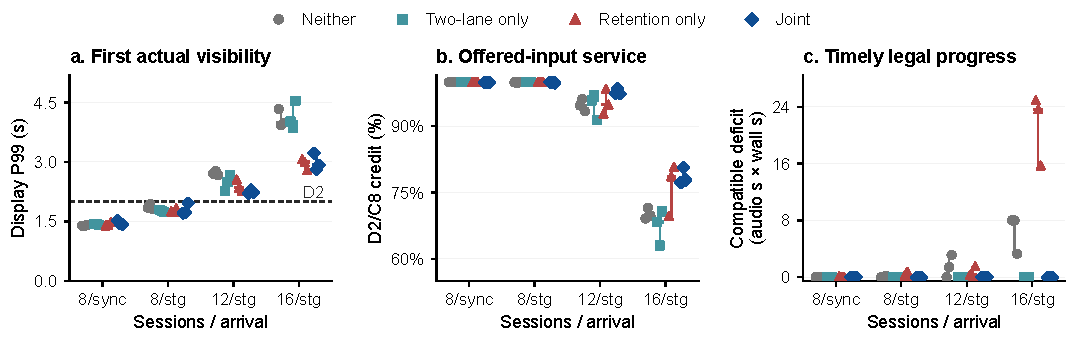
\includegraphics[width=\textwidth]{figures/service_region.pdf}
\caption{All four development workloads and three fresh-process runs per
arm, including the negative twelve-session midpoint. Points are real
per-run values; ticks and ranges describe their median and observed
range. Panel~(c) is the separate secondary measure of subsequent
compatible loss of originally timely intervals, censored at the next
Canonical root when necessary. It does not replace panel~(b)'s original
first-observation credit.}
\label{fig:service-region}
\end{figure*}

All arms pass whole-run D2/C8 in the two eight-session workloads.
Joint display P99 is 1.426--1.528~s when synchronized, where the arms
largely converge. Staggered joint P99 reaches 1.955~s, and an earlier
development run reached 2.034~s, exposing a narrow timing margin.
Two 0.215-s tails exceed D2 in the new eight-session runs and remain
uncredited even though their runs' P99 passes. At sixteen sessions,
all twelve runs fail D2, while C8 passes. Joint credit exceeds $R_0S_0$
by 20.280/22.885/20.180~s, but its credit interactions are
$+20.910$, $+26.380$, and $-9.575$~s.
Against computation-only, joint credit changes by
$+18.910$, $+5.055$, and $-7.225$~s, and display P99 improves
in only one repeat. Continuity is the stable distinction: computation-only
withdraws compatible views 16/17/12 times, versus zero for joint.

First credit does not reveal a later withdrawal. A frozen secondary
recount therefore follows intervals already delivered within D2 whose
eventual certified covering view also meets C8. At each subsequent
Canonical application it classifies withdrawal using the complete old
view's dependency witness, separately recording necessary incompatible
withdrawals. Loss lasts until an actual covering view returns or the
next Canonical boundary censors this root's window. At sixteen sessions,
computation-only still has 10/12/9 timely compatible loss windows with
24.903/23.635/15.736 audio-s$\times$wall-s deficit area; joint has none.
Such holes intersect the original D2 read point for 6.000/10.675/4.000~s
of distinct audio. The secondary measures continuity after delivery;
it neither changes Eq.~\eqref{eq:credit} nor certifies provisional content.

The twelve-session midpoint sought a stronger witness: both
computation-only and joint must pass whole-run D2/C8 in all three
repeats, computation-only must lose an originally timely complete 2-s
non-EOS interval in at least two, and joint must have no compatible
timely loss. This witness is \emph{not established}. All twelve
midpoint runs fail D2; joint P99 is 2.197/2.299/2.228~s.
Computation-only has 1/1/3 timely loss windows, but none qualifies as
a complete non-EOS interval. Joint has zero, yet cannot turn this into
a successful whole-run operating point. The predeclared stop rule
closes this exploration without another session count or extra repeats.

\subsection{Quality and cost boundaries}
All headline Qwen arms have WER $26/1908=1.36\%$ and identical selected
histories. Retrospective support counting first-certified content plus
first-ahead whole views that exactly match later same-$F$ Canonical
text leaves the headline credits unchanged. Elsewhere raw differences
remain: joint loses 2~s of strict support in the sixteen-session third
repeat and 2~s in each of the midpoint's first two repeats, although
the frozen text normalizer agrees. This comparison is with the selected
model output, not human-transcription correctness. Whisper exposes a
larger adapter boundary: WER is 83.12\% at $\rho=1$ and 11.53\% at
$\rho=3$, whose different feedback contract prevents interpreting it
as a quality-preserving speedup.

The headline arms consume similar board energy (Table~\ref{tab:core-h3});
energy does not rank them in credit order. At sixteen development
sessions, joint reduces total model time by 0.66--1.59~s against $R_0S_0$,
while serving wall time does not consistently fall and the
three energy differences change sign. The measured benefit is the
progress delivered and preserved under a fixed feedback contract.
It is not a general reduction in inference cost or a cure for overload.

% Complete service evidence; component, development and independent scopes stay separate.
\subsection{Native correction with the original selected task}
\label{subsec:native_retention_eval}
We retain StreamCorrect's published recognizer, learned correction, and
feedback update~\cite{vu2026streamcorrect}, using the fixed 500-ms, no-VAD
adaptation and original FP32 execution. Both compared policies have two
protected full workers, the same ASR early-view Consumer, and identical
neural warmup. Conservative execution waits for selected parent feedback
before starting the next call; full-call retention confirms conditional
calls as in Section~\ref{subsec:native_full_calls}.

\paragraph{Development and frozen confirmation}
Component controls cover all 69 steps of four AISHELL-1 utterances used
for implementation development~\cite{bu2017aishell}: 65 complete ASR
packets reproduce original $C/U$, with four buffer-only steps using the
original path. Thirteen identity-projected ends differ from selection
without invalidating that candidate input. Comparison with the earlier
implementation removes only the newly added implementation-contract tag;
complete task state, corrections, and returned IDs remain equal.

A three-arm source-0 pilot gives conservative execution, already-ready
ASR handoff, and conditional full calls 3.0, 6.5, and 8.0~s of original
credit over 8.068~s offered. Full calls can retain work still executing
when its input is confirmed; ready-only handoff requires a complete
received packet. We select our full-call implementation and confirm it
with 16 runs on all four development sources. These are development
measurements, including two 0.068-s EOS misses, rather than independent
acoustic evidence.

We then freeze that method before selecting four previously unused
AISHELL-1 speakers using archive metadata and an 8--9-s duration band.
All four initial selections remain; no model output selects a source.
The final experiment has four separate chains, two fresh-process repeats,
and two policies: 16 runs. Paired arm order reverses on the second repeat,
GPU roles swap, and pair blocks are randomized. The independent acoustic
unit is a speaker, not a repeat or offered frontier. All original
500-ms frontiers and partial EOS intervals stay in the denominator.

\paragraph{Task fidelity and timely service}
Offline original full calls supply 68 reference transitions, separately
from service timing. All 272 Canonical transitions in the new experiment reproduce
their complete original start and end states, $C$, and returned IDs,
including the implementation tag. Both arms have five character edits
over 81 unique reference characters, or 6.17\% CER; across repeated flows
the equivalent count is 10/162. This measures the adaptation, not the
published author's benchmark CER. Development runs separately preserve
all 276 transitions and have 16/182 repeated-character edits.

\begin{table}[t]
\centering
\caption{Native service: eight runs per arm in each panel. Offered audio
per arm is 66.430~s for development and 66.340~s for independent sources.
Credit and energy are totals; C50 is the median of per-run C50 values.
Text support compares the first actual whole view at $G$ with later
complete Canonical text at exactly $G$. Values are rounded.}
\label{tab:native_full_confirm}
\small
\setlength{\tabcolsep}{2.5pt}
\begin{tabular}{@{}lrrrrr@{}}
\toprule
Policy & \shortstack{Credit\\(s)} & \shortstack{Text\\support (s)} &
\shortstack{C50\\(s)} & \shortstack{Energy\\(kJ)} & Pass\\
\midrule
\multicolumn{6}{@{}l}{Development: four existing sources}\\
Conservative & 37.500 & 33.500 & 1.905 & 36.942 & 0/8\\
Full-call & 66.294 & 56.288 & 1.035 & 32.050 & 6/8\\
\midrule
\multicolumn{6}{@{}l}{Independent: four new speakers}\\
Conservative & 37.000 & 29.000 & 2.115 & 35.801 & 0/8\\
Full-call & 66.340 & 51.518 & 1.203 & 31.815 & 8/8\\
\bottomrule
\end{tabular}
\end{table}

Table~\ref{tab:native_full_confirm} keeps development and independent
results separate. On new speakers, credit increases in all eight pairs,
from 37.0 to all 66.33975~s offered per arm. All four speakers have a
positive two-repeat sum, satisfying the frozen directional rule; this is
not an eight-independent-sample significance test. Full-call retention
passes whole-run D2/C8 in 8/8 runs, versus 0/8. Its D99 ranges from 0.837
to 1.663~s and C99 from 1.090 to 1.929~s. It has no D2 or C8 miss;
conservative execution has 62 D2 misses, including eight EOS intervals,
and no C8 miss. The median per-run C50 falls from 2.115 to 1.203~s.
Both-board serving energy, excluding loading and fixed neural warmup,
falls 11.13\%; credit, C50, and energy improve in every pair.

\paragraph{Retained work and visible content}
Ninety-two promoted calls are actually computing before their selected
parent finishes, and their model intervals overlap the parent's. Twenty
have their own identity-predicted end differ from original correction.
Twenty-four calls stop after ASR under invalidity or coverage proofs,
before $C/U$; two
already-completed conditional full results are discarded. None changes
the original selected history. These observations distinguish input
confirmation from requiring each future prediction to be correct.

The new runs also contain a concrete whole-view witness: one Canonical
application advances from 4.0 to 4.5~s while retaining a supported 5.0-s
Private view and its original executing call. Two other applications,
on one speaker's two repeats, withdraw 6.0 to 5.5~s because the call's
complete predicted input disagrees with the actual selected state;
the two complete conditional results are not installed. These natural
events illustrate compatible retention and necessary withdrawal, not
another factorial estimate of the $R\times S$ interaction.

Posterior whole-text support remains separate from original credit.
Supported credited audio increases from 29.0 to 51.518125~s in all eight
pairs; raw and whitespace-only comparisons agree and unknown coverage
is zero. The remaining 14.821625~s of full-call credit does not have this
support. Six of eight first EOS texts differ from later Canonical text
in each arm. These are selected-model comparisons, not human correctness
certificates. Both arms introduce 180 LCP-versioned codepoint occurrences,
retract 14, and end with 166 across eight flows. Unchanged-text rows first
cover 10.0 versus 17.0 credited audio seconds; processing-frontier credit
does not count newly transcribed characters.

An earlier two-source capacity experiment retains its negative result:
retention earns 17.0~s versus 18.5~s for independent full replicas, using
47.991 versus 25.949~kJ. Its warmup and Consumer differ. The present
single-chain comparison establishes a service opportunity in this scope;
it neither supplies a causal before/after comparison nor establishes
superior saturated multi-source capacity.

% Selected execution support from the earlier combined draft; native evidence is separate.
% Completed K24, exact-F support96, and native14 only; no stage-profile or handoff result.
\subsection{From physical release to supported service}
\label{subsec:release_evidence}
We isolate computation retention $R$ and coverage exit $K$ while enabling
the legal two-lane Consumer $S$ in every arm. The study uses the same
executor, 16 fixed development sources, and 250.180\,s of offered audio per
run. Four arms, synchronized or staggered arrivals, and three fresh-process
repetitions give 24 runs. A frozen wrong-conditioning fixture supplies
controlled useless tails. It is separate from the unmodified-input work
used to establish lawful continuation. Original input obligations, D2/C8
deadlines, quality, and physical costs remain unchanged.

All selected Canonical $F/Z/P/T$ histories match, with WER $14/687$ in
every run. All 675 pairs with identical complete processed inputs,
actual prompt/audio identities, and peer order return identical outputs.

Each synchronized $K1$ run releases a following batch of 16 rows that
matches its $K0$ counterpart on these inputs and outputs. Under $R1$, the
following model computation starts 473/577/498\,ms earlier across the three
repetitions. Request, acknowledgment, and drain remain distinct: in one
repeat, request-to-ACK is 22.196\,ms and ACK-to-actual-drain is 13.359\,ms.
All 96 following rows across the six synchronized comparisons are actually
consumed and first advance their target frontiers.

Canonical may already cover an obsolete proposal, so obsolescence alone
does not establish a missed deadline. Comparing actual first coverage
from either lane, only 6/6/1 rows under $R1$ and 4/2/6 under $R0$ change
from dual-deadline miss to hit. All 96 first-consumed hypotheses agree
byte-for-byte with later complete Canonical text at exactly the same
frontier, and their worker records contain no input override. This
retrospective selected-model agreement supplies content support for the
newly timely rows; it is not an online content certificate or human
transcription accuracy.

The whole-run boundary is less uniform. Adding $K$ to $R1$ increases
original credit by 15.255/13.265/7.970 audio seconds under synchronized
arrivals, but changes it by $-26.000/-6.475/+21.780$\,s under staggered
arrivals. Neither whole-run model time nor board energy improves
consistently. Whole-run first content remains revisable: each synchronized
arm has 16\,s of timely first-ahead content differing from later
same-frontier Canonical text, or 14\,s after the fixed normalizer. These
equal deductions leave the synchronized credit differences intact.
We therefore use simple coverage exit as execution support, with a
measured drain-to-service chain, rather than a universally beneficial
cancellation algorithm or a stable positive $R\times K$ interaction.


\section{Related Work}\label{sec:related}
\paragraph{Incremental information and dependency reuse}
The incremental-unit model separates newest committed information from
the active right edge and propagates dependency revocation
\cite{schlangen2011incremental}. Its commit promises that a unit will not
be revoked. Here, certification records acceptance by the protected
selection protocol; later selected facts may still revise the transcript.
Adapton checks recorded dependencies; Nominal Adapton combines names with
arguments and dependency checks to recover reusable work
\cite{hammer2014adapton,hammer2015names}. Differential Dataflow maintains
incremental computations across evolving versions
\cite{mcsherry2013differential}. These works establish much of the basis for
dependency-aware reuse. RevTrace instantiates that basis for complete
neural feedback state and frozen executed calls. Its service obligation
connects execution eligibility to the actual whole view retained when an
independently selected root is applied.
Our sufficient witness follows recorded executions; it does not transfer a
from-scratch theorem to independently repeated floating-point inference.

\paragraph{Revisable speech services and speculation}
Whisper-Streaming converts an offline recognizer into incremental service
using LocalAgreement~\cite{machacek2023whisperstreaming}. StreamCorrect
adds learned correction and feeds selected corrections into subsequent
recognition~\cite{vu2026streamcorrect}. RevTrace retains that selection and
feedback behavior in its controlled native adapter; its contribution
concerns the asynchronous execution and consumption around the feedback
boundary. It does not introduce a better acoustic model or train a new
corrector.

SSBD coordinates old-output draft reuse with display-only suffix masking
\cite{zeng2026ssbd}. It revalidates a draft under updated input and includes
an unbiased configuration. RevTrace follows complete calls that actually
executed to establish their eligibility under newly selected feedback state,
then checks the dependency witness for the Consumer's whole current view.
PredGen provides a close precedent for speculation while speech input
evolves across recognition, language generation, and speech synthesis
\cite{li2025predgen}. Our comparison holds the complete selected feedback
task fixed across the retention policies. The specific reuse object,
protected selection, and whole-view transition define the composition
evaluated here. RelayS2S uses a learned verifier to commit a fast-path
prefix that constrains subsequent slow-path generation
\cite{mai2026relays2s}. Our native calls instead confirm their complete
inputs and retain the original correction and feedback update. Work on
ASR alignment drift also establishes the importance and cost of audio
position state~\cite{wang2026alignmentdrift}; our contract includes that
state rather than treating text equality as sufficient.

\paragraph{Execution, authorization, and recovery}
Retire studies versioned execution and bounded physical exit for
interruptible agents~\cite{zhang2026retire}. RevTrace likewise distinguishes
logical progress from an executor's actual release, while deriving the
tested retention and coverage decisions from the feedback contract. Our
simple covered-exit implementation is execution support, without a claim
to a new general cancellation algorithm. A parent-version cancellation
control is not a reproduction of the complete Retire system.

Optimistic and multiversion concurrency control separate validation and
commit from concurrent execution~\cite{kung1981occ,bernstein1983mvcc}.
Write-ahead recovery persists state changes and identities
\cite{mohan1992aries}, and stream-processing systems coordinate recoverable
state~\cite{carbone2017flinkstate}. We use these established principles at
the ASR feedback boundary. They supply machinery for ordering and
durability; the adapter still has to specify which state constitutes a
valid continuation and which complete view the Consumer may retain.

\section{Discussion}\label{sec:discussion}
\paragraph{Scope of the guarantee}
The continuation witness assumes a sufficient adapter state and faithful
execution of frozen inputs. A new adapter must account for every mutable
field that can affect later inference, selection, or feedback. A hidden
KV cache, alignment cursor, or external tool state can invalidate a
token-only argument. Conservative rejection remains allowed when a
sufficient witness is absent. The guarantee concerns dependency validity
and an individual compatible application; it supplies neither transcription
correctness nor monotone text for an entire session.

\paragraph{Progress, content, and capacity}
Processing more audio can leave the cumulative transcript unchanged.
Frontier credit, actual text additions and revisions, eventual selected
text agreement, and ground-truth accuracy answer different questions. We
report them with their original denominators. Preserving compatible
progress also cannot remove all input synchronization, queueing, or neural
work. The negative c12 witness and the native two-replica comparison
identify concrete limits of this implementation rather than a universal
capacity envelope. The independent native confirmation establishes a
single-chain service opportunity with the original selected task; it
does not turn that result into saturated multi-source capacity.

\paragraph{Deployment and validation}
The prototype evaluates short streams selected before inference and does not
establish bounded memory or long-running collection of dependency history.
Production deployment would also require network-facing delivery and
ownership transfer beyond the local FIFO Consumer. Our crash evidence uses
an earlier frozen recovery prototype on intact storage; it is not a
full-stack proof for every later runtime or native adapter. The artifact
separates source-level controls, bounded protocol exploration, controlled
faults, actual GPU service, and retrospective analyses so their evidence
roles remain inspectable.

\section{Conclusion}\label{sec:conclusion}
RevTrace preserves dependency-valid speculative work and whole delivered
hypotheses while trusted feedback continues to advance. Its explicit
feedback contract supports executable re-rooting witnesses, coordinated
computation and consumption, and separate physical retirement. Actual
service experiments show that first delivery can meet its deadline while
subsequent compatible updates withdraw the delivered progress. The joint
design preserves the whole ahead view at compatible root applications,
with necessary revisions, execution costs, and capacity limits kept visible.
The core experiments show why retaining computation does not itself
preserve already delivered service. The native implementation confirms a
call's complete input and retains original correction work without requiring
its own next prediction to be correct. Together, these results establish
a concrete composition of dependency reuse, protected feedback, and
whole-view consumption, with measured timing and capacity boundaries.

\section*{AI Tool Usage}
ChatGPT/Codex assisted literature discovery, experiment orchestration,
analysis and validation code, manuscript drafting, and figures. The artifact
records execution sources, frozen configurations, controls, and result
provenance, and distinguishes actual service measurements from component
tests and retrospective analyses. The authors retain responsibility for the
submission.
\clearpage
\bibliographystyle{IEEEtran}
\bibliography{refs,formal_refs,coordination_refs}
\end{document}
